\documentclass[oneside, mag]{mgr}	
 
\usepackage{polski}	
\usepackage[utf8]{inputenc}	
\usepackage{amsmath}		
\usepackage{graphicx}	
\graphicspath{ {./} }
\usepackage{amsfonts}
\usepackage{hyperref}
\usepackage{tabstackengine}
\usepackage{caption}
\usepackage{subfig}
\usepackage{listings}

\newcommand{\bb}{\textbf}

\title{Analiza efektywności zastosowania sieci rekurencyjnych w zadaniu klasyfikacji}	
\engtitle{Analysis of the effectiveness of recursive networks in the classification task}
\author{Jędrzej Kozal}
\supervisor{dr  inż. Paweł Ksieniewicz}

\field{Informatyka (Inf)}
\specialisation{Systemy informatyki w medycynie (IMT)}

\begin{document}
\bibliographystyle{plabbrv}	

\maketitle

\tableofcontents

\chapter{Wstęp}

W niniejszym rozdziale zarysowano problematykę pracy i pokrótce omówiono zagadnienia, które będą wykorzystywane w dalszej części. Dokonano przeglądu literaturowego i opisano plan badań.

\section{Wprowadzenie}

\subsection{Sieci neuronowe}

\begin{figure}
	\centering
	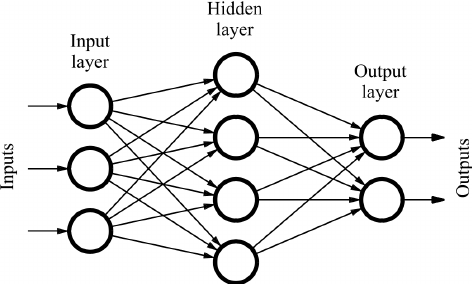
\includegraphics[scale=0.7]{img/feed-forward-nn.png}
	\caption{Schemat sieci neuronowej} Źródło: https://www.researchgate.net/profile/Ramon\_Quiza/publication/234055177/figure/fig1/\\AS:300092981563410@1448559150651/Sample\-of\-a\-feed\-forward-neural\-network.png
	\label{feedforward-NN}
\end{figure}

Sieci neuronowe to szeroka klasa modeli wykorzystywana najczęściej do zadania uczenia nadzorowanego. W podstawowej formie sieć składa się z wielu warstw neuronów połączonych ze sobą (zob rys. \ref{feedforward-NN}). Warstwa wejściowa sieci odpowiada za przyjmowanie wektorów wejściowych. Neurony w warstwie ukrytej realizują funkcję nieliniową opisaną równaniem:

\begin{equation}
	x_i = f(w_i u_i)
\end{equation}

Gdzie $x_i$ jest wyjściem $i$-tego neuronu w warstwie (nazywanym również aktywacją neuronu), $f$ jest funkcją aktywacji w warstwie do której należy neuron, $w_i$ jest wektorem wag $i$-tego neuronu a $u_i$ jest wektorem wejść $i$-tego neuronu. Nieliniowość operacji jest powodowana przez nieliniową funkcję aktywacji. W procesie uczenia definiowana jest funkcja strat (loss function) $L$ opisująca w sposób ilościowy jak bardzo wyjście sieci neuronowej różni się od oczekiwanej wartości. Wartości funkcji strat są wykorzystywane do modyfikacji wag sieci neuronowej (algorytm wstecznej propagacji błędu), najczęściej z wykorzystaniem reguł gradientowych. Dzięki algorytmowi wstecznej propagacji możliwe jest uczenie wielowarstwowych sieci. Wyjście każdej warstwy stanowi zmodyfikowaną reprezentację oryginalnej przestrzeni. Dzięki nieliniowości i tworzeniu reprezentacji przestrzeni cech, sieci neuronowe potrafią generować bardzo złożone granice decyzyjne.

Sieci neuronowe są starą klasą modeli. Pierwsze prace w zakresie reguł uczenia pojawiły się latach 40 XX wieku \cite{McCulloch-Pitts} \cite{Hebb}. Rosenblat \cite{Rosenblatt} skonstruował perceptron - maszynę wykazującą zdolność nauki. Uważa się, że publikacja w które zbadano ogarniczenia perpceptoronu i udowodniono, że podejedyncza wartswa sieci nie jest w stanie nauczyć się funkcji XOR \cite{Perceptrons} zaczpoątkowała okres nazwany zimą sztucznej inteligencji (AI Winter). Prawdziwym przełomem okazała się praca \cite{Rumelhart} w której zaproponowano algorytm wstecznej propagacji błędów. Po tej publikacji zainteresowanie głębokimi sieciami neuronowymi zaczęło wzrastać. W \cite{Conv} zaproponowano warstwy konwolucyjne, które pozwoliły na łatwiejsze przetwarzanie obrazów przez sieci neuronowe. 
Gwałtowny wzrost popularności sieci neuronowych w ostatnich latach można przypisać kilku czynnikom \cite{Goodfellow-et-al-2016}. Pierwszym z nich jest zwiększenie mocy obliczeniowej dostępnej dla praktyków i badaczy uczenia maszynowego, co pozwoliło na zwiększenie rozmiarów modeli i skrócenie czasu uczenia. Drugim czynnikiem jest pojawienie wielu obszernych zbiorów danych, powodowane przez rozpowszechnienie się internetu i urządzeń elektronicznych w życiu codziennym ludzi. Oba te czynniki pozwalają na skuteczne trenowanie modeli o większych pojemnościach, do coraz bardziej złożonych zadań.

Można dopatrywać się powiązań między sposobem działania ludzkiego mózgu a sieciami neuronowymi. Podobieństwo to może być widoczne przy sposobie działania synaps komórki nerowowej. Badacze podkreślają \cite{Goodfellow-et-al-2016}, że związek sieci neuronowych z biologią ma bardziej charakter luźnej inspiracji niż rzeczywistego modelu zjawisk zachodzących w ludzkim mózgu.

\subsection{Rekurencyjne sieci neuronowe}

\begin{figure}
	\centering
	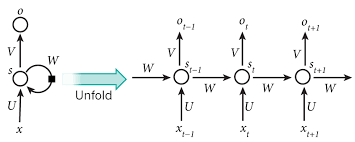
\includegraphics[scale=1.0]{img/rnn.png}
	\caption{Schemat sieci rekurencyjnej.} Źródło: http://www.wildml.com/2015/09/recurrent-neural-networks-tutorial-part-1-introduction-to-rnns/ (Lewo) sieci rekurencyjne można przedstawić jako jednostkę obliczeniową, która do realizacji obliczeń wykorzystuje wartości uzyskane dla poprzednich kroków. Na rysunku jest to widoczne w formie czarnego kwadratu, oznaczającego opóźnienie czasowe o jeden krok przy neuronie obok normalnych wejść i wyjść. (Prawo) rozwinięta wersja tego samego schematu, przedstawiająca w jaki sposób obliczenia są wykonywane w poszczególnych krokach. Reprezentacja ta pozwala na łatwiejszą analizę zachowań sieci i stosowanych algorytmów. 
	\label{fig:rnn}
\end{figure}

Sieci feedforward posiadają stałą liczbę wejść i wyjść, przez co nie radzą sobie dobrze z przetwarzaniem danych występujących w ciągach (takich jak tekst, dźwięki czy ciągi czasowe). Istnieją podejścia umożliwiające przetwarzanie ciągów przez sieci feedforward, ale nie są one skuteczne. W celu zaadresowania tego problemu powstały sieci rekurencyjne (Recurrent Neural Networks - RNN).
Sieci Rekurencyjne zostały oparte na pracy Rumelharta \cite{RNN}. RNN posiadają ukryty stan, będący warstwą ukrytą sieci, którego wartość jest obliczana nie tylko na podstawie aktualnego wejścia, ale też na podstawie poprzedniego stanu sieci (zob rys. \ref{fig:rnn}).
Algorytm uczenia RNN - propagacja wsteczna w czasie (Back-Propagation Through Time - BPTT) zostały przedstawione w \cite{BPTT}.
Udowodniono, że przy pewnych założeniach RNN są kompletne w sensie Turinga \cite{turing-complete}.

\subsubsection{Sieci dwukierunkowe}

Wprowadzono wiele modyfikacji w zakresie zasad działania i strukturze RNN. 
W \cite{bidirectional} wprowadzono sieci dwukierunkowe, przetwarzające sekwencje w dwóch kierunkach: od początku do końca sekwencji i od końca do początku. Ostateczna wartość dla n-tego elementu sekwencji jest obliczana na podstawie n-tego wyniku dla obu kierunków.

\subsubsection{LSTM}

RNN w swojej natywnej formie nie są w stanie nauczyć się długich zależności w ciągu uczącym. Problem ten jest w znacznej mierze spowodowany wybuchającymi lub znikającymi gradientami (exploding or vanishing gradients \cite{vanishing_gradient_RNN}). W celu zaadresowania tego problemu Hochreiter i Schmidhuber zaproponowali architekturę Long Short-Term Memory (LSTM) \cite{LSTM}. Ze względu na swoją strukturę LSTM jest w stanie operować na danych z długimi zależnościami czasowymi. LSTM jest dokładniej opisane w późniejszej części pracy. 

\subsubsection{GRU}

Gated Recurrent Unit (GRU) \cite{DBLP:journals/corr/ChungGCB15} jest modyfikacją LSTM. Podstawowa zasada działania modelu zostaje taka sama. Wprowadzone zmiany dotyczą struktury sieci i polegają na zastosowaniu dwóch zamiast trzech komórek, co powoduje zmniejszenie liczby parametrów. Mniejsza liczba parametrów przekłada się na zmniejszenie wymagań w zakresie mocy obliczeniowej potrzebnych do nauczenia modelu, co może mieć przełożenie na zwiększenie głębokości modelu lub zwiększenie ukrytych jednostek. Z drugiej strony zmniejszenie liczby bramek powoduje zmniejszenie mocy modelu. Z praktycznego punktu widzenia LSTM i GRU uzyskują porównywalne wyniki \cite{DBLP:journals/corr/ChungGCB14}.

\subsubsection{Neuronowe Maszyny Turinga}

Rozwinięciem idei wykorzystania pamięci do usprawnienia działania sieci są Neuronowe Maszyny Turinga \cite{DBLP:journals/corr/GravesWD14}. Neuronowe Maszyny Turinga korzystają z mechanizmu uwagi do operacji na pamięci. Pamięć przypomina pamięć dostępną w komputerze i składa się z wielu wektorów, które można wykorzystać do odczytu lub przechowywania informacji. Neuronowa Maszyna Turinga posiada dwie głowice: do zapisu i odczytu. Adresowanie pamięci odbywa się na podstawie zawartości (content-base addressing) lub położenia (location-base addressing).

\subsection{Zadanie klasyfikacji}

Uczenie nadzorowane (ang. supervised learning) to dział uczenia maszyn w którym zbiór uczący składa się z par $\{x, d\}_{i=1}^N$, gdzie $x$ to wektor cech, $d$ to etykieta, a $N$ to liczność zbioru uczącego. W przypadku gdy każdej cechy istnieje osobna etykieta mówimy o silnym etykietowaniu. Gdy jedna etykieta opisuje wszystkie cechy z przykładu uczącego mówimy o słabym etykietowaniu. Przykładowo jeśli zadanie polega na rozpoznaniu, że na zdjęciu znajduje się samochód mówimy o słabym etykietowaniu. Jeśli zadanie polega na zaznaczeniu wszystkich pikseli przedstawiających samochód na zdjęciu, mówimy o silnym etykietowaniu. Aby określić jakość działania algorytmu wprowadza się funkcję straty dla całego zbioru:

\begin{equation}
	\mathcal{L} = \sum_{i=1}^N L_i
\end{equation}

Zadanie klasyfikacji opiera się na przypisaniu przykładu uczącego $x$ do odpowiedniej klasy $k$. W procesie uczenia wybieramy hipotezę z przestrzeni hipotez $h \in \mathcal{H}$, która minimalizuje liczbę błędnie zaklasyfikowanych przykładów \cite{introduction-to-machine-learning}. Można to zapisać za pomocą 0-1 funkcji strat:

\begin{equation}
	E(x, d) = \sum_{i=1}^N 1(h(x_i) \neq d_i )
\end{equation}

gdzie $1(x)$ jest równe 1, gdy x jest prawdziwe i 0 gdy x nie jest prawdziwe. 0-1 funkcja strat może być stosowana, gdy na wyjściu klasyfikatora znajduje się etykieta klasy. W przypadku gdy na wyjściu modelu znajduje się prawdopodobieństwo przynależności do klasy często stosowana jest entropia krzyżowa (ang cross entropy):

\begin{equation}
	H(h,d) = - \sum h(x) log(d)
\end{equation}

Reguła decyzyjna w takim przypadku opiera się na wyborze najbardziej prawdopodobnej klasy:

\begin{equation}
	h(x) = arg \; \stackunder{max}{k} \; p(C_k | x)
\end{equation}

gdzie $x_i$ to $i$-ty element wektora, będącego argumentem funkcji softmax.

W przypadku sieci neuronowych często stosowaną mechaniką jest wykorzystywanie funkcji softmax w warstwie wyjściowej sieci. Funkcja softmax pozwala na konwertowanie wyjść sieci na prawdopodobieństwa i jest dana wzorem:

\begin{equation}
	softmax(x)_i = \frac{e^{x_i}}{\sum_{k=1}^{K} e^{x_k}}
\end{equation}

Algorytmy klasyfikacji dostosowane dla sieci rekurencyjnych takie jak Connectionist Temporal
Classification zostały szczegółowo omówione w \cite{graves-phd}. W przypadku tej pracy ich wymaganie nie będzie wskazane, ze względu na charakter wykorzystanej architektury sieci.

\section{Przegląd literatury}

W \cite{DBLP:journals/corr/VisinKCMCB15} wykorzystano sieć rekurencyjną do klasyfikacji obrazów i porównano uzyskane wyniki z rezultatami dla sieci konwolucyjnych. Proponowany model (ReNet) wykorzystywał RNN do czterotnego trawersowania fragmentów obrazu w celu ekstrakcji cech, jako alternatywę dla warstw konwolucyjnych z poolingiem. W \cite{DBLP:journals/corr/KalchbrennerDG15} przedstawiono GRID LSTM, które rozszerzało standardowy model sieci LSTM do N-wymiarowych komórek ze współdzielonymi wektorami stanu i pamięci.

\subsection{Zastosowania rekurencyjnych sieci neuronowych}

Sieci Rekurencyjne znalazły wiele zastosowań w przetwarzaniu sekwencji. 
Jednym z takich zastosowań może być przetwarzanie języka naturalnego (natural language processing - NLP), gdzie RNN znalazły zastosowanie w rozpoznawaniu mowy \cite{DBLP:journals/corr/abs-1303-5778}, \cite{speech_recognition}, \cite{speech_recognition1}, tłumaczeniu \cite{translate}, \cite{DBLP:journals/corr/ChoMGBSB14}, \cite{DBLP:journals/corr/BahdanauCB14}, \cite{DBLP:journals/corr/WuSCLNMKCGMKSJL16}, modelowniu języka \cite{DBLP:journals/corr/ChoMGBSB14}, generowaniu mowy \cite{DBLP:journals/corr/MehriKGKJSCB16} i generowaniu tekstu \cite{DBLP:journals/corr/Graves13} \cite{karpathy_RNN_blog}. 
Innym polem zastosowań RNN jest rozpoznawanie pisma ręcznego \cite{handwriting_recognition}, \cite{handwriting_recognition2} lub jego generacja \cite{DBLP:journals/corr/Graves13}.
RNN są także wykorzystywane do generowania obrazów \cite{DBLP:journals/corr/GregorDGW15} i muzyki \cite{DBLP:journals/corr/abs-1804-07300}.
Autorzy \cite{DBLP:journals/corr/VinyalsL15} zaproponowali system do przeprowadzania rozmóm zbudowany z wykorzystaniem RNN. 
W \cite{sentiment_analysis} wykorzystano RNN do analizy sentymentu.

Sieci rekurencyjne są także wykorzystywane w połączeniu z innymi modelami np. CNN w przypadku generowania podpisów dla obrazów \cite{DBLP:journals/corr/VinyalsTBE14}, gdzie CNN jest wykorzystywane do klasyfikacji obrazu i przygotowywania reprezentacji obrazu w architekturze encoder-decoder, a RNN generuje podpis obrazka.

\section{Cel pracy}

Celem pracy jest zbadanie skuteczności klasyfikacji zmodyfikowanej architektury sieci ReNet. Proponowana modyfikacja polega na zastąpieniu czterech sieci rekurencyjnych jedną dwukierunkową siecią rekurencyjną analizącą obraz jednowymiarowy ciąg otrzymany z wykorzystaniem krzywych wypełniającej przestrzeń (ang. space-filling curves). Wyniki klasyfikacji wybranego zbioru danych zostaną porównane z oryginalną architekturą oraz wynikami osiąganymi dla sieci konwolucyjnych. Wykorzystanie jednej sieci rekurencyjnej powinno pozwolić na zmniejszenie liczby parametrów modelu, co może przekładać się na krótszy czas szkolenia. W zakres badań będzie wchodziło również wpływ wyboru krzywej wypełniającej przestrzeń oraz różnych architektur sieci rekurencyjnych na uzyskiwane wyniki. Ze względu na ograniczoną dostępną moc obliczeniową hiperparametry modeli zostaną dobrane z wykorzystaniem podziału zbioru danych na zbiór uczący i zbiór testowy oraz wykorzystaniem algorytmu wyszukiwania sieciowego (ang. grid search). Dokładność klasyfikacji zostanie zmierzona z wykorzystaniem dokładności (accuracy)

\chapter{Omówienie wybranych zagadnień teoretycznych}

W niniejszym rozdziale zostały omówione teoretyczne podstawy wybranych algorytmów i struktur sieci, które zostały wykorzystane w badaniach.

\section{Rekurencyjna Sieć Neuronowa}

\section{Propagacja wsteczna w czasie}

\section{LSTM}

\begin{figure}
\centering
	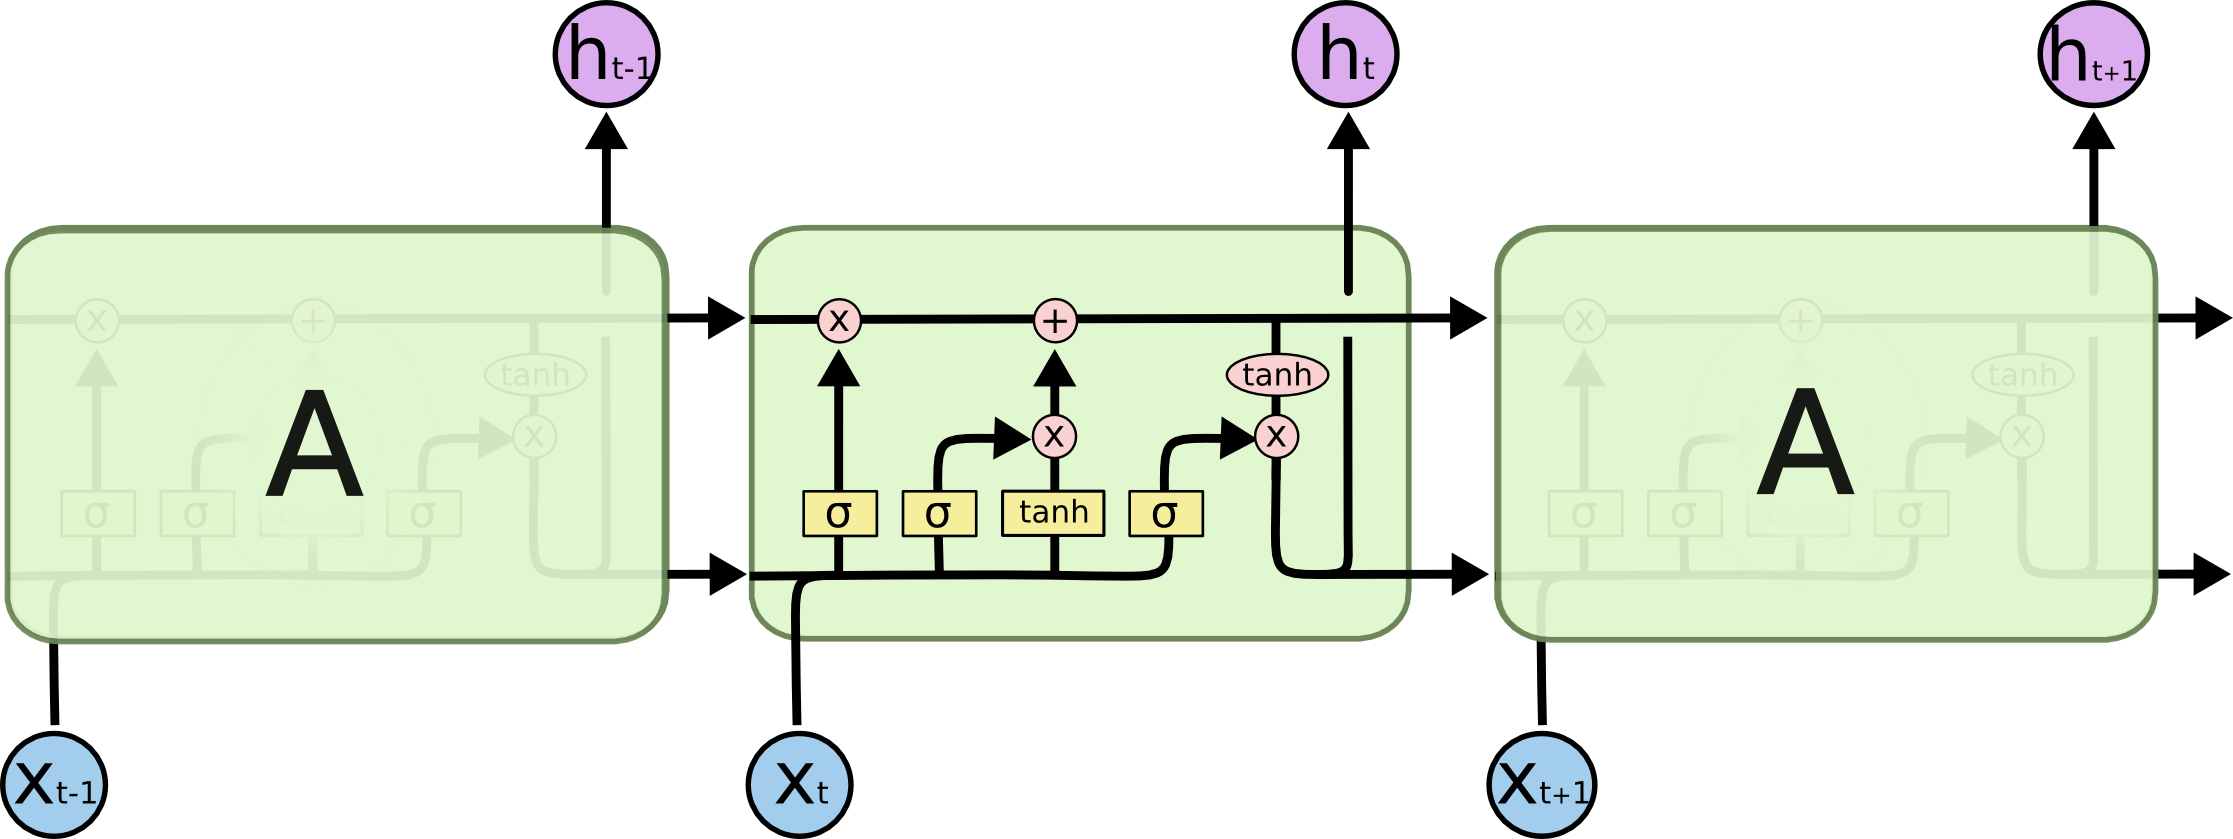
\includegraphics[width=0.90\textwidth]{img/lstm_colah.png}
	\caption{Schemat komórki LSTM.} Źródło: http://colah.github.io/posts/2015-08-Understanding-LSTMs/
	\label{fig:lstm}
\end{figure}

LSTM jest jedną z popularniejszych architektur RNN. Hochreiter i Schmidhuber zaproponowali architekturę Long Short-Term Memory (LSTM) \cite{LSTM} w 1997. Zwykła sieć RNN składa się jedynie ze stanu sieci $h$, oraz wejścia $x$, które są wejściem warstwy ukrytej sieci. Wyjście warstwy ukrytej jest wyjściem sieci. Struktura komórki LSTM jest bardziej skomplikowana i składa się z wektora stanu sieci $h$, komórki pamięci $C$, oraz czterech ukrytych warstw sieci. Schemat ze strukturą sieci został przedstawiony na rys. \ref{fig:lstm}.

Warstwy sieci LSTM z sigmoidalnymi funkcjami aktywacji są nazywane bramkami multiplikatywnymi. Sigmoidalna funkcja aktywacji jest opisywana za pomocą wzoru:

\begin{equation}
	\sigma(x) = \frac{1}{e^{-x} + 1}
\end{equation}

i posiada zbiór wartości $(0, 1)$. Przemnożenie wyjścia tej warstwy z dowolną wartością powoduje jej przeskalowanie, przez co warstwy te są wykorzystywane do kontrolowania wartości zmiennych komórki LSTM. Dodatkowo bramki jako warstwy sieci posiadają wagi, które ulegają modyfikacji w trakcie uczenia, przez co LSTM w procesie uczenia zyskują informację o tym kiedy i w jaki sposób uaktualnić swój stan i komórkę pamięci na podstawie obecnie posiadanych informacji. Wyróżnia się 3 bramki. Pierwszą z nich jest forget gate. Jest ona odpowiedzialna za zmniejszanie wartości aktualnie znajdującej się w komórce pamięci. Operacja realizowana przez forget gate jest opisywana wzorem: 

\begin{equation}
	f_t = \sigma( W_f [ h_{t-1}, x_t ] + b_f )
\end{equation}

Gdzie $W_f$ i $b_f$ to odpowiednio wagi i bias warstwy, $h_{t-1}$ to stan komórki z poprzedniego kroku, a $x_t$ to aktualne wejście sieci. Kolejną bramką jest input gate. Realizowana operacja wyraża się analogicznym wzorem:

\begin{equation}
	i_t = \sigma( W_i [ h_{t-1}, x_t ] + b_i )
\end{equation}

Intuicyjnie jest ona odpowiedzialna za określanie w jakim stopniu należy zaktualizować komórkę pamięci sieci na podstawie aktualnego wejścia sieci $x_t$ i stanu z poprzedniego kroku $h_{t-1}$. Na podstawie $x_t$ i $h_{t-1}$ jest obliczana wartość $\tilde{C}_t$:

\begin{equation}
	\tilde{C}_t = tanh( W_c [ h_{t-1}, x_t ] + b_C )
\end{equation}

Wartość $\tilde{C}_t$ może być określona jako kandydat do zastąpienia stanu komórki z poprzedniego kroku $C_{t-1}$. Aktualna wartość $C_t$ jest zatem obliczana ze wzoru:

\begin{equation}
	C_t = f_t \odot C_{t-1} + i_t \odot \tilde{C}_t
\end{equation}

gdzie $\odot$ oznacza iloczyn Hadamarda (iloczyn wszystkich elementów wektora lub macierzy). Ostatnią bramką jest output gate. Realizowana operacja jest dana wzorem:

\begin{equation}
	o_t = \sigma( W_o [ h_{t-1}, x_t ] + b_o )
\end{equation}

Służy do określania, sposobu w jaki zostanie zaktualizowany stan $h$ w aktualnym kroku $t$, co wyraża się równaniem:

\begin{equation}
	h_t = o_t \odot tanh( C_t )
\end{equation}

\begin{figure}
\centering
	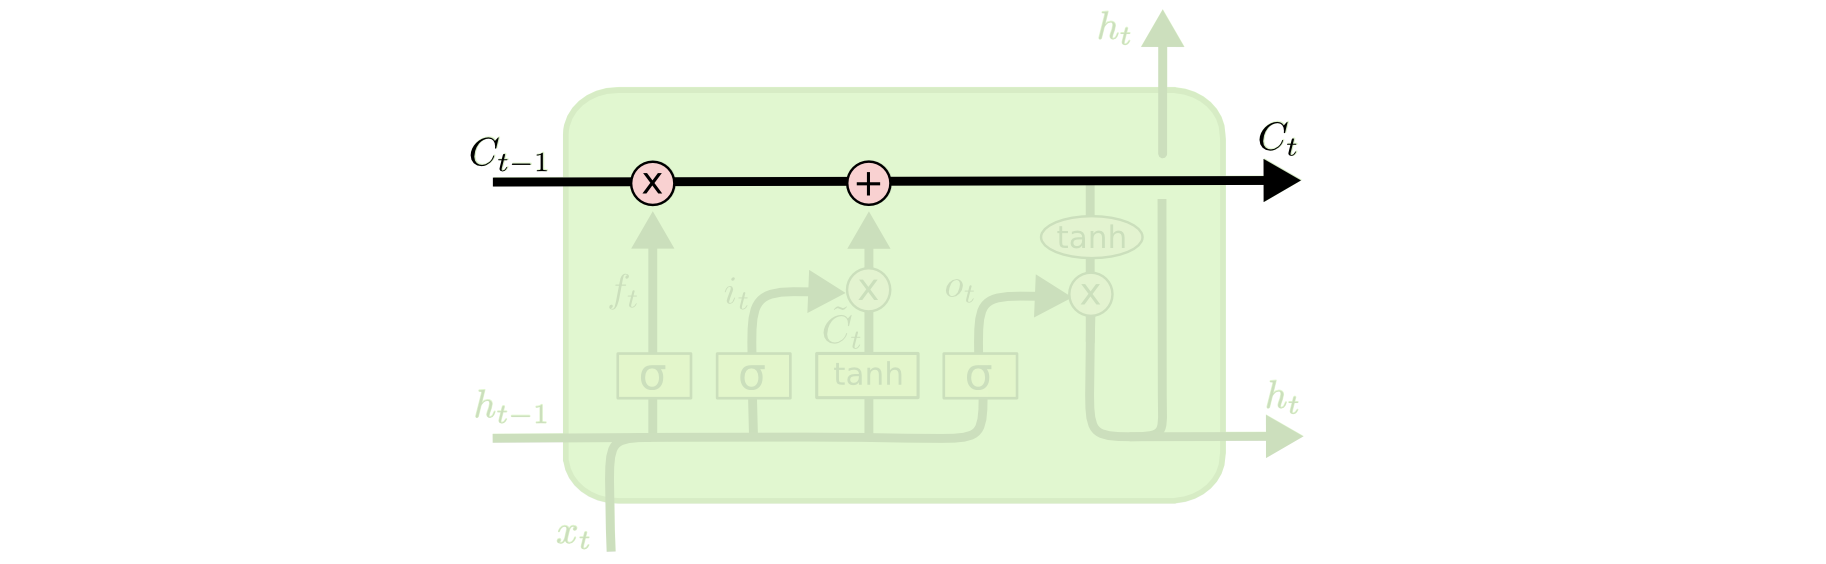
\includegraphics[width=0.90\textwidth]{img/LSTM3-C-line.png}
	\caption{Schemat komórki LSTM z zaznaczoną komórką pamięci.} Źródło: http://colah.github.io/posts/2015-08-Understanding-LSTMs/. W przypadku propagacji wstecznej przy cofaniu się przez graf obliczeniowy sieci węzły odpowiadające operacji dodawania propagują wartość błędu bez modyfikacji wartości. Węzły w grafie odpowiadające operacji mnożenia powodują przemnożenie wartości dotychczasowego błędu przez drugi argument. W tym przypadku realizowana operacja to $C_t = f_t \odot C_{t-1} + i_t \odot \tilde{C}_t$. W wyniku propagacji wstecznej uzyskujemy pochodną $\frac{\partial L}{\partial C_t}$. Opearcja dodawnia nie zmienia wartość błędu, więc $\frac{\partial L}{\partial (f_t \odot C_{t-1})} = \frac{\partial L}{\partial C_t}$. Przy operacji mnożenia pochodna cząstkowa względem $C_{t-1}$ wynosi $\frac{\partial C_t}{\partial C_{t-1}} = f_t$. Błąd propagowany przez komórkę pamięci ma ostateczną wartość: $\frac{\partial L}{\partial C_{t-1}} = \frac{\partial L}{\partial C_t} f_t$. Ze względu na zbiór wartości funkcji sigmoidalnej $f_t \in (0, 1)$ wartość propagowanego błędu nadal jest pomniejszana w każdym kroku. Intuicyjnie wartość błędu jest zmniejszana w takim samym stopniu jak wartość sygnału przy normalnym przejściu przez forget gate (decyzja w jakim stopniu informacje nie są istotne w aktualnym kontekście). Zaproponowana architektura unika jednakże obliczania pochodnej względem funkcji aktywacji sigmoidalnej (pochodna funkcji sigmoidalnej: $\frac{d \sigma}{dx} = \sigma (x)(1 - \sigma (x)$) przy propagacji wstecznej błędu, co powoduje wolniejsze zmniejszanie wartości sygnału błędu. 
	\label{fig:lstm-mem-cell}
\end{figure}

Warto zwrócić uwagę, że w powyższym równaniu nie występują wagi ani bias, więc $tanh$ nie jest utożsamiony z warstwą sieci neuronowej.

W swojej pracy \cite{LSTM} Hochreiter i Schmidhuber odnoszą się do wcześniejszej pracy \cite{vanishing_gradient_RNN}, gdzie zostały przeanalizowane źródła problemów związanych ze znikającymi gradientami. Jako główny problem został wskazany gradient względem dowolnej zmiennej w grafie $a$ obliczeniowym $|\frac{\partial L}{\partial a}| > 1.0$ powodujący wybuchanie wag, lub $|\frac{\partial L}{\partial a}| < 1.0$ powodujący znikanie wag. W strukturze LSTM komórka pamięci jest sposobem zapobiegania temu problemowi. Komórka pamięci przy propagacji wstecznej pozwala na swobodniejszą propagację błędu wiele kroków wstecz, dzięki czemu sieć w procesie uczenia jest w stanie uwzględnić długie zależności czasowe (zob rys. \ref{fig:lstm-mem-cell}). Kolejnym problemem związanym z uczeniem zwykłych RNN jest otrzymywanie sprzecznych sygnałów przy aktualizacji wag. W przypadku gdzie ta sama warstwa sieci neuronowej jest odpowiedzialna za określenie w jakim stopniu stan sieci z poprzedniego kroku jest nadal istotny, oraz w jakim stopniu można wykorzystać aktualną wartość stanu sieci, uczenie sieci może być trudne. W LSTM ten problem został rozwiązany przez wyodrębnienie warstw odpowiedzialnych za osobne operacje.  

\section{GRU}

\begin{figure}
\centering
	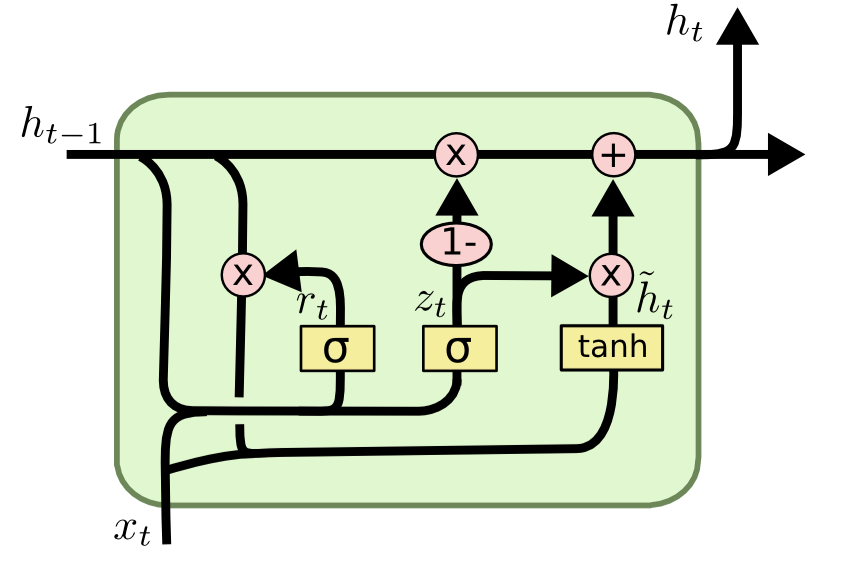
\includegraphics[width=0.5\textwidth]{img/LSTM3-var-GRU.png}
	\caption{Schemat komórki GRU.} Źródło: http://colah.github.io/posts/2015-08-Understanding-LSTMs/
	\label{fig:gru}
\end{figure}

\chapter{Problem badawczy}

\section{ReNet}

\section{Proponowana architektura sieci}

\section{Krzywe wypełniające przestrzeń}




\chapter{Przeprowadzone badania}

\section{Metodyka badań}

\section{Opis eksperymentu}

\subsection{Zbiór danych}

\subsection{Wykorzystane narzędzia i hardware}

\subsection{Dobór hiperparametrów modelu}



\chapter{Wyniki}


\chapter{Wnioski}

\bibliography{bibliography}

\listoffigures

\end{document}